\section*{Výsledky měření}
Teplota v místnosti a tedy i teplota roztoků byla \SI{21.7(3)}{\degreeCelsius}.




Jako silný elektrolyt jsme použili \SI{0.01}{M} HCl a jako slabý jsme použili \SI{0.01}{M} \ce{CH_3COOH}.

Změřili jsme měrnou elektrickou vodivost destilované vody.
Měrnou vodivost destilované vody použité k~přípravě roztoků jsme změrili dvakrát, ještě před měřením roztoků HCl jsme naměřili \SI{1.35}{\micro\siemens\per\centi\metre}, poté mezi měřením HCl a \ce{CH_3COOH} jsme naměřili \SI{1.37}{\micro\siemens\per\centi\metre}.
Tyto hodnoty jsou také uvedeny v prvním řádku tabulky~\ref{t:vysledky}.
Po měření \ce{CH_3COOH} destilovaná voda došla a byla doplněna jinou, konduktivitu jsme změřili \SI{1.23}{\micro\siemens\per\centi\metre}

Výsledky jsou shrnuty v tabulce \ref{t:vysledky}.
První sloupec ($V$) udává, jaký objem roztoku jsme napipetovali do baňky a poté doplnili na \SI{100}{\milli\litre}.
Molární koncentraci vypočteme
\begin{equation*}
c_M = \frac{V}{\SI{100}{\milli\litre}} \cdot \SI{0.01}{M}
\end{equation*}

Při měření jsme počkali, než se hodnota na konduktometru ustálí. Používali jsme konduktometr Mettler Toledo s přesností \SI{0.5}{\percent}.

\begin{tabulka}[htbp]
\centering
\begin{tabular}{cc|cc|cc}
 & & \multicolumn{2}{c|}{\ce{HCl}} & \multicolumn{2}{c}{\ce{CH_3COOH}} \\
$V$ (\si{\milli\litre}) & $c_M$ (\si{\mol\per\metre\cubed}) & $\sigma$ (\si{\micro\siemens\per\centi\metre}) & $\Lambda$ (\si{\milli\siemens\metre\squared\per\mol}) & $\sigma$ (\si{\micro\siemens\per\centi\metre}) & $\Lambda$ (\si{\milli\siemens\metre\squared\per\mol}) \\
\hline
0  & \num{0.0} & \num{1.35} & --- & \num{1.37} & --- \\
1  & \num{0.1} & \num{37.8} & \num{37.8} & \num{12.6} & \num{12.6} \\
2  & \num{0.2} & \num{74.8} & \num{37.4} & \num{20.4} & \num{10.2} \\
4  & \num{0.4} & \num{148} & \num{37.0} & \num{29.4} & \num{7.35} \\
6  & \num{0.6} & \num{221} & \num{36.8} & \num{36.4} & \num{6.07} \\
8  & \num{0.8} & \num{303} & \num{37.9} & \num{42.5} & \num{5.31} \\
10 & \num{1.0} & \num{375} & \num{37.5} & \num{47.7} & \num{4.77} \\
\end{tabular}
\caption{}
\label{t:vysledky}
\end{tabulka}


\begin{graph}[htbp] 
\centering
% GNUPLOT: LaTeX picture with Postscript
\begingroup
  \makeatletter
  \providecommand\color[2][]{%
    \GenericError{(gnuplot) \space\space\space\@spaces}{%
      Package color not loaded in conjunction with
      terminal option `colourtext'%
    }{See the gnuplot documentation for explanation.%
    }{Either use 'blacktext' in gnuplot or load the package
      color.sty in LaTeX.}%
    \renewcommand\color[2][]{}%
  }%
  \providecommand\includegraphics[2][]{%
    \GenericError{(gnuplot) \space\space\space\@spaces}{%
      Package graphicx or graphics not loaded%
    }{See the gnuplot documentation for explanation.%
    }{The gnuplot epslatex terminal needs graphicx.sty or graphics.sty.}%
    \renewcommand\includegraphics[2][]{}%
  }%
  \providecommand\rotatebox[2]{#2}%
  \@ifundefined{ifGPcolor}{%
    \newif\ifGPcolor
    \GPcolorfalse
  }{}%
  \@ifundefined{ifGPblacktext}{%
    \newif\ifGPblacktext
    \GPblacktexttrue
  }{}%
  % define a \g@addto@macro without @ in the name:
  \let\gplgaddtomacro\g@addto@macro
  % define empty templates for all commands taking text:
  \gdef\gplbacktext{}%
  \gdef\gplfronttext{}%
  \makeatother
  \ifGPblacktext
    % no textcolor at all
    \def\colorrgb#1{}%
    \def\colorgray#1{}%
  \else
    % gray or color?
    \ifGPcolor
      \def\colorrgb#1{\color[rgb]{#1}}%
      \def\colorgray#1{\color[gray]{#1}}%
      \expandafter\def\csname LTw\endcsname{\color{white}}%
      \expandafter\def\csname LTb\endcsname{\color{black}}%
      \expandafter\def\csname LTa\endcsname{\color{black}}%
      \expandafter\def\csname LT0\endcsname{\color[rgb]{1,0,0}}%
      \expandafter\def\csname LT1\endcsname{\color[rgb]{0,1,0}}%
      \expandafter\def\csname LT2\endcsname{\color[rgb]{0,0,1}}%
      \expandafter\def\csname LT3\endcsname{\color[rgb]{1,0,1}}%
      \expandafter\def\csname LT4\endcsname{\color[rgb]{0,1,1}}%
      \expandafter\def\csname LT5\endcsname{\color[rgb]{1,1,0}}%
      \expandafter\def\csname LT6\endcsname{\color[rgb]{0,0,0}}%
      \expandafter\def\csname LT7\endcsname{\color[rgb]{1,0.3,0}}%
      \expandafter\def\csname LT8\endcsname{\color[rgb]{0.5,0.5,0.5}}%
    \else
      % gray
      \def\colorrgb#1{\color{black}}%
      \def\colorgray#1{\color[gray]{#1}}%
      \expandafter\def\csname LTw\endcsname{\color{white}}%
      \expandafter\def\csname LTb\endcsname{\color{black}}%
      \expandafter\def\csname LTa\endcsname{\color{black}}%
      \expandafter\def\csname LT0\endcsname{\color{black}}%
      \expandafter\def\csname LT1\endcsname{\color{black}}%
      \expandafter\def\csname LT2\endcsname{\color{black}}%
      \expandafter\def\csname LT3\endcsname{\color{black}}%
      \expandafter\def\csname LT4\endcsname{\color{black}}%
      \expandafter\def\csname LT5\endcsname{\color{black}}%
      \expandafter\def\csname LT6\endcsname{\color{black}}%
      \expandafter\def\csname LT7\endcsname{\color{black}}%
      \expandafter\def\csname LT8\endcsname{\color{black}}%
    \fi
  \fi
  \setlength{\unitlength}{0.0500bp}%
  \begin{picture}(6802.00,3968.00)%
    \gplgaddtomacro\gplbacktext{%
      \csname LTb\endcsname%
      \put(946,704){\makebox(0,0)[r]{\strut{} 0}}%
      \csname LTb\endcsname%
      \put(946,1079){\makebox(0,0)[r]{\strut{} 50}}%
      \csname LTb\endcsname%
      \put(946,1454){\makebox(0,0)[r]{\strut{} 100}}%
      \csname LTb\endcsname%
      \put(946,1829){\makebox(0,0)[r]{\strut{} 150}}%
      \csname LTb\endcsname%
      \put(946,2204){\makebox(0,0)[r]{\strut{} 200}}%
      \csname LTb\endcsname%
      \put(946,2578){\makebox(0,0)[r]{\strut{} 250}}%
      \csname LTb\endcsname%
      \put(946,2953){\makebox(0,0)[r]{\strut{} 300}}%
      \csname LTb\endcsname%
      \put(946,3328){\makebox(0,0)[r]{\strut{} 350}}%
      \csname LTb\endcsname%
      \put(946,3703){\makebox(0,0)[r]{\strut{} 400}}%
      \csname LTb\endcsname%
      \put(1078,484){\makebox(0,0){\strut{} 0}}%
      \csname LTb\endcsname%
      \put(2047,484){\makebox(0,0){\strut{} 0.2}}%
      \csname LTb\endcsname%
      \put(3015,484){\makebox(0,0){\strut{} 0.4}}%
      \csname LTb\endcsname%
      \put(3984,484){\makebox(0,0){\strut{} 0.6}}%
      \csname LTb\endcsname%
      \put(4952,484){\makebox(0,0){\strut{} 0.8}}%
      \csname LTb\endcsname%
      \put(5921,484){\makebox(0,0){\strut{} 1}}%
      \put(176,2203){\rotatebox{-270}{\makebox(0,0){\strut{}$\sigma$ (\si{\micro\siemens\per\centi\metre})}}}%
      \put(3741,154){\makebox(0,0){\strut{}$c_M$ (\si{\mol\per\metre\cubed})}}%
    }%
    \gplgaddtomacro\gplfronttext{%
      \csname LTb\endcsname%
      \put(5418,1555){\makebox(0,0)[r]{\strut{}\ce{HCl}}}%
      \csname LTb\endcsname%
      \put(5418,1240){\makebox(0,0)[r]{\strut{}$375\cdot x$}}%
      \csname LTb\endcsname%
      \put(5418,925){\makebox(0,0)[r]{\strut{}$384\cdot x-\num{21.2} \cdot x^{1.5}$}}%
    }%
    \gplbacktext
    \put(0,0){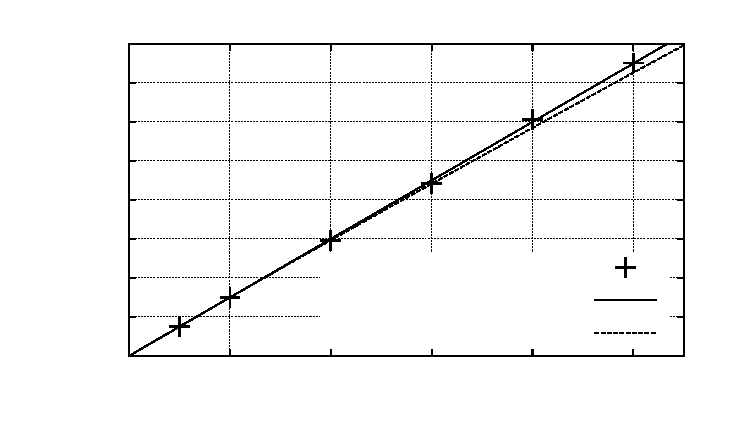
\includegraphics{sCl}}%
    \gplfronttext
  \end{picture}%
\endgroup

\caption{Závislost konduktivity \ce{HCl} na koncentraci}
\label{g:sCl}
\end{graph}

\begin{graph}[htbp] 
\centering
% GNUPLOT: LaTeX picture with Postscript
\begingroup
  \makeatletter
  \providecommand\color[2][]{%
    \GenericError{(gnuplot) \space\space\space\@spaces}{%
      Package color not loaded in conjunction with
      terminal option `colourtext'%
    }{See the gnuplot documentation for explanation.%
    }{Either use 'blacktext' in gnuplot or load the package
      color.sty in LaTeX.}%
    \renewcommand\color[2][]{}%
  }%
  \providecommand\includegraphics[2][]{%
    \GenericError{(gnuplot) \space\space\space\@spaces}{%
      Package graphicx or graphics not loaded%
    }{See the gnuplot documentation for explanation.%
    }{The gnuplot epslatex terminal needs graphicx.sty or graphics.sty.}%
    \renewcommand\includegraphics[2][]{}%
  }%
  \providecommand\rotatebox[2]{#2}%
  \@ifundefined{ifGPcolor}{%
    \newif\ifGPcolor
    \GPcolorfalse
  }{}%
  \@ifundefined{ifGPblacktext}{%
    \newif\ifGPblacktext
    \GPblacktexttrue
  }{}%
  % define a \g@addto@macro without @ in the name:
  \let\gplgaddtomacro\g@addto@macro
  % define empty templates for all commands taking text:
  \gdef\gplbacktext{}%
  \gdef\gplfronttext{}%
  \makeatother
  \ifGPblacktext
    % no textcolor at all
    \def\colorrgb#1{}%
    \def\colorgray#1{}%
  \else
    % gray or color?
    \ifGPcolor
      \def\colorrgb#1{\color[rgb]{#1}}%
      \def\colorgray#1{\color[gray]{#1}}%
      \expandafter\def\csname LTw\endcsname{\color{white}}%
      \expandafter\def\csname LTb\endcsname{\color{black}}%
      \expandafter\def\csname LTa\endcsname{\color{black}}%
      \expandafter\def\csname LT0\endcsname{\color[rgb]{1,0,0}}%
      \expandafter\def\csname LT1\endcsname{\color[rgb]{0,1,0}}%
      \expandafter\def\csname LT2\endcsname{\color[rgb]{0,0,1}}%
      \expandafter\def\csname LT3\endcsname{\color[rgb]{1,0,1}}%
      \expandafter\def\csname LT4\endcsname{\color[rgb]{0,1,1}}%
      \expandafter\def\csname LT5\endcsname{\color[rgb]{1,1,0}}%
      \expandafter\def\csname LT6\endcsname{\color[rgb]{0,0,0}}%
      \expandafter\def\csname LT7\endcsname{\color[rgb]{1,0.3,0}}%
      \expandafter\def\csname LT8\endcsname{\color[rgb]{0.5,0.5,0.5}}%
    \else
      % gray
      \def\colorrgb#1{\color{black}}%
      \def\colorgray#1{\color[gray]{#1}}%
      \expandafter\def\csname LTw\endcsname{\color{white}}%
      \expandafter\def\csname LTb\endcsname{\color{black}}%
      \expandafter\def\csname LTa\endcsname{\color{black}}%
      \expandafter\def\csname LT0\endcsname{\color{black}}%
      \expandafter\def\csname LT1\endcsname{\color{black}}%
      \expandafter\def\csname LT2\endcsname{\color{black}}%
      \expandafter\def\csname LT3\endcsname{\color{black}}%
      \expandafter\def\csname LT4\endcsname{\color{black}}%
      \expandafter\def\csname LT5\endcsname{\color{black}}%
      \expandafter\def\csname LT6\endcsname{\color{black}}%
      \expandafter\def\csname LT7\endcsname{\color{black}}%
      \expandafter\def\csname LT8\endcsname{\color{black}}%
    \fi
  \fi
  \setlength{\unitlength}{0.0500bp}%
  \begin{picture}(6802.00,3968.00)%
    \gplgaddtomacro\gplbacktext{%
      \csname LTb\endcsname%
      \put(814,704){\makebox(0,0)[r]{\strut{} 35}}%
      \csname LTb\endcsname%
      \put(814,1304){\makebox(0,0)[r]{\strut{} 36}}%
      \csname LTb\endcsname%
      \put(814,1904){\makebox(0,0)[r]{\strut{} 37}}%
      \csname LTb\endcsname%
      \put(814,2503){\makebox(0,0)[r]{\strut{} 38}}%
      \csname LTb\endcsname%
      \put(814,3103){\makebox(0,0)[r]{\strut{} 39}}%
      \csname LTb\endcsname%
      \put(814,3703){\makebox(0,0)[r]{\strut{} 40}}%
      \csname LTb\endcsname%
      \put(946,484){\makebox(0,0){\strut{} 0}}%
      \csname LTb\endcsname%
      \put(1939,484){\makebox(0,0){\strut{} 0.2}}%
      \csname LTb\endcsname%
      \put(2931,484){\makebox(0,0){\strut{} 0.4}}%
      \csname LTb\endcsname%
      \put(3924,484){\makebox(0,0){\strut{} 0.6}}%
      \csname LTb\endcsname%
      \put(4916,484){\makebox(0,0){\strut{} 0.8}}%
      \csname LTb\endcsname%
      \put(5909,484){\makebox(0,0){\strut{} 1}}%
      \put(176,2203){\rotatebox{-270}{\makebox(0,0){\strut{}$\Lambda$ (\si{\milli\siemens\metre\squared\per\mol})}}}%
      \put(3675,154){\makebox(0,0){\strut{}$\sqrt{c_M}$ ($(\si{\mol\per\metre\cubed})^{1/2}$)}}%
    }%
    \gplgaddtomacro\gplfronttext{%
      \csname LTb\endcsname%
      \put(2926,1555){\makebox(0,0)[r]{\strut{}\ce{HCl}}}%
      \csname LTb\endcsname%
      \put(2926,1240){\makebox(0,0)[r]{\strut{}\num{37.4}}}%
      \csname LTb\endcsname%
      \put(2926,925){\makebox(0,0)[r]{\strut{}$\num{38.4}-\num{2.12}\cdot x$}}%
    }%
    \gplbacktext
    \put(0,0){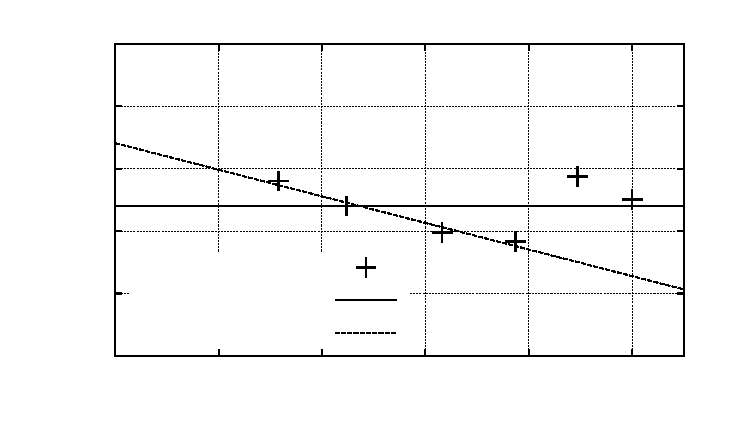
\includegraphics{lCl}}%
    \gplfronttext
  \end{picture}%
\endgroup

\caption{Závislost molární konduktivity \ce{HCl} na odmocnině z koncentrace}
\label{g:lCl}
\end{graph}

\begin{graph}[htbp] 
\centering
% GNUPLOT: LaTeX picture with Postscript
\begingroup
  \makeatletter
  \providecommand\color[2][]{%
    \GenericError{(gnuplot) \space\space\space\@spaces}{%
      Package color not loaded in conjunction with
      terminal option `colourtext'%
    }{See the gnuplot documentation for explanation.%
    }{Either use 'blacktext' in gnuplot or load the package
      color.sty in LaTeX.}%
    \renewcommand\color[2][]{}%
  }%
  \providecommand\includegraphics[2][]{%
    \GenericError{(gnuplot) \space\space\space\@spaces}{%
      Package graphicx or graphics not loaded%
    }{See the gnuplot documentation for explanation.%
    }{The gnuplot epslatex terminal needs graphicx.sty or graphics.sty.}%
    \renewcommand\includegraphics[2][]{}%
  }%
  \providecommand\rotatebox[2]{#2}%
  \@ifundefined{ifGPcolor}{%
    \newif\ifGPcolor
    \GPcolorfalse
  }{}%
  \@ifundefined{ifGPblacktext}{%
    \newif\ifGPblacktext
    \GPblacktexttrue
  }{}%
  % define a \g@addto@macro without @ in the name:
  \let\gplgaddtomacro\g@addto@macro
  % define empty templates for all commands taking text:
  \gdef\gplbacktext{}%
  \gdef\gplfronttext{}%
  \makeatother
  \ifGPblacktext
    % no textcolor at all
    \def\colorrgb#1{}%
    \def\colorgray#1{}%
  \else
    % gray or color?
    \ifGPcolor
      \def\colorrgb#1{\color[rgb]{#1}}%
      \def\colorgray#1{\color[gray]{#1}}%
      \expandafter\def\csname LTw\endcsname{\color{white}}%
      \expandafter\def\csname LTb\endcsname{\color{black}}%
      \expandafter\def\csname LTa\endcsname{\color{black}}%
      \expandafter\def\csname LT0\endcsname{\color[rgb]{1,0,0}}%
      \expandafter\def\csname LT1\endcsname{\color[rgb]{0,1,0}}%
      \expandafter\def\csname LT2\endcsname{\color[rgb]{0,0,1}}%
      \expandafter\def\csname LT3\endcsname{\color[rgb]{1,0,1}}%
      \expandafter\def\csname LT4\endcsname{\color[rgb]{0,1,1}}%
      \expandafter\def\csname LT5\endcsname{\color[rgb]{1,1,0}}%
      \expandafter\def\csname LT6\endcsname{\color[rgb]{0,0,0}}%
      \expandafter\def\csname LT7\endcsname{\color[rgb]{1,0.3,0}}%
      \expandafter\def\csname LT8\endcsname{\color[rgb]{0.5,0.5,0.5}}%
    \else
      % gray
      \def\colorrgb#1{\color{black}}%
      \def\colorgray#1{\color[gray]{#1}}%
      \expandafter\def\csname LTw\endcsname{\color{white}}%
      \expandafter\def\csname LTb\endcsname{\color{black}}%
      \expandafter\def\csname LTa\endcsname{\color{black}}%
      \expandafter\def\csname LT0\endcsname{\color{black}}%
      \expandafter\def\csname LT1\endcsname{\color{black}}%
      \expandafter\def\csname LT2\endcsname{\color{black}}%
      \expandafter\def\csname LT3\endcsname{\color{black}}%
      \expandafter\def\csname LT4\endcsname{\color{black}}%
      \expandafter\def\csname LT5\endcsname{\color{black}}%
      \expandafter\def\csname LT6\endcsname{\color{black}}%
      \expandafter\def\csname LT7\endcsname{\color{black}}%
      \expandafter\def\csname LT8\endcsname{\color{black}}%
    \fi
  \fi
  \setlength{\unitlength}{0.0500bp}%
  \begin{picture}(6802.00,3968.00)%
    \gplgaddtomacro\gplbacktext{%
      \csname LTb\endcsname%
      \put(814,704){\makebox(0,0)[r]{\strut{} 0}}%
      \csname LTb\endcsname%
      \put(814,1304){\makebox(0,0)[r]{\strut{} 10}}%
      \csname LTb\endcsname%
      \put(814,1904){\makebox(0,0)[r]{\strut{} 20}}%
      \csname LTb\endcsname%
      \put(814,2503){\makebox(0,0)[r]{\strut{} 30}}%
      \csname LTb\endcsname%
      \put(814,3103){\makebox(0,0)[r]{\strut{} 40}}%
      \csname LTb\endcsname%
      \put(814,3703){\makebox(0,0)[r]{\strut{} 50}}%
      \csname LTb\endcsname%
      \put(946,484){\makebox(0,0){\strut{} 0}}%
      \csname LTb\endcsname%
      \put(1939,484){\makebox(0,0){\strut{} 0.2}}%
      \csname LTb\endcsname%
      \put(2931,484){\makebox(0,0){\strut{} 0.4}}%
      \csname LTb\endcsname%
      \put(3924,484){\makebox(0,0){\strut{} 0.6}}%
      \csname LTb\endcsname%
      \put(4916,484){\makebox(0,0){\strut{} 0.8}}%
      \csname LTb\endcsname%
      \put(5909,484){\makebox(0,0){\strut{} 1}}%
      \put(176,2203){\rotatebox{-270}{\makebox(0,0){\strut{}$\sigma$ (\si{\micro\siemens\per\centi\metre})}}}%
      \put(3675,154){\makebox(0,0){\strut{}$c_M$ (\si{\mol\per\metre\cubed})}}%
    }%
    \gplgaddtomacro\gplfronttext{%
      \csname LTb\endcsname%
      \put(5418,1555){\makebox(0,0)[r]{\strut{}\ce{CH_3COOH}}}%
      \csname LTb\endcsname%
      \put(5418,1240){\makebox(0,0)[r]{\strut{}$\num{5}\cdot (\sqrt{1+100\cdot x}-1)+\num{1.37}$}}%
      \csname LTb\endcsname%
      \put(5418,925){\makebox(0,0)[r]{\strut{}$\num{155}\cdot x - \num{115} \cdot x^{3/2}$}}%
    }%
    \gplbacktext
    \put(0,0){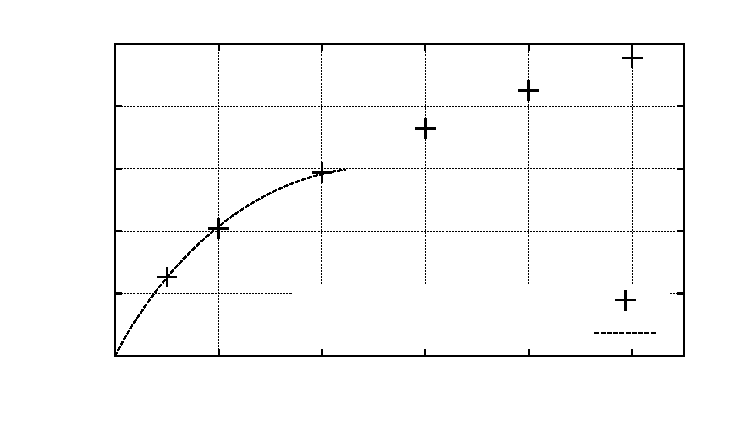
\includegraphics{sCH}}%
    \gplfronttext
  \end{picture}%
\endgroup

\caption{Závislost konduktivity \ce{CH_3COOH} na koncentraci}
\label{g:sCH}
\end{graph}

\begin{graph}[htbp] 
\centering
% GNUPLOT: LaTeX picture with Postscript
\begingroup
  \makeatletter
  \providecommand\color[2][]{%
    \GenericError{(gnuplot) \space\space\space\@spaces}{%
      Package color not loaded in conjunction with
      terminal option `colourtext'%
    }{See the gnuplot documentation for explanation.%
    }{Either use 'blacktext' in gnuplot or load the package
      color.sty in LaTeX.}%
    \renewcommand\color[2][]{}%
  }%
  \providecommand\includegraphics[2][]{%
    \GenericError{(gnuplot) \space\space\space\@spaces}{%
      Package graphicx or graphics not loaded%
    }{See the gnuplot documentation for explanation.%
    }{The gnuplot epslatex terminal needs graphicx.sty or graphics.sty.}%
    \renewcommand\includegraphics[2][]{}%
  }%
  \providecommand\rotatebox[2]{#2}%
  \@ifundefined{ifGPcolor}{%
    \newif\ifGPcolor
    \GPcolorfalse
  }{}%
  \@ifundefined{ifGPblacktext}{%
    \newif\ifGPblacktext
    \GPblacktexttrue
  }{}%
  % define a \g@addto@macro without @ in the name:
  \let\gplgaddtomacro\g@addto@macro
  % define empty templates for all commands taking text:
  \gdef\gplbacktext{}%
  \gdef\gplfronttext{}%
  \makeatother
  \ifGPblacktext
    % no textcolor at all
    \def\colorrgb#1{}%
    \def\colorgray#1{}%
  \else
    % gray or color?
    \ifGPcolor
      \def\colorrgb#1{\color[rgb]{#1}}%
      \def\colorgray#1{\color[gray]{#1}}%
      \expandafter\def\csname LTw\endcsname{\color{white}}%
      \expandafter\def\csname LTb\endcsname{\color{black}}%
      \expandafter\def\csname LTa\endcsname{\color{black}}%
      \expandafter\def\csname LT0\endcsname{\color[rgb]{1,0,0}}%
      \expandafter\def\csname LT1\endcsname{\color[rgb]{0,1,0}}%
      \expandafter\def\csname LT2\endcsname{\color[rgb]{0,0,1}}%
      \expandafter\def\csname LT3\endcsname{\color[rgb]{1,0,1}}%
      \expandafter\def\csname LT4\endcsname{\color[rgb]{0,1,1}}%
      \expandafter\def\csname LT5\endcsname{\color[rgb]{1,1,0}}%
      \expandafter\def\csname LT6\endcsname{\color[rgb]{0,0,0}}%
      \expandafter\def\csname LT7\endcsname{\color[rgb]{1,0.3,0}}%
      \expandafter\def\csname LT8\endcsname{\color[rgb]{0.5,0.5,0.5}}%
    \else
      % gray
      \def\colorrgb#1{\color{black}}%
      \def\colorgray#1{\color[gray]{#1}}%
      \expandafter\def\csname LTw\endcsname{\color{white}}%
      \expandafter\def\csname LTb\endcsname{\color{black}}%
      \expandafter\def\csname LTa\endcsname{\color{black}}%
      \expandafter\def\csname LT0\endcsname{\color{black}}%
      \expandafter\def\csname LT1\endcsname{\color{black}}%
      \expandafter\def\csname LT2\endcsname{\color{black}}%
      \expandafter\def\csname LT3\endcsname{\color{black}}%
      \expandafter\def\csname LT4\endcsname{\color{black}}%
      \expandafter\def\csname LT5\endcsname{\color{black}}%
      \expandafter\def\csname LT6\endcsname{\color{black}}%
      \expandafter\def\csname LT7\endcsname{\color{black}}%
      \expandafter\def\csname LT8\endcsname{\color{black}}%
    \fi
  \fi
  \setlength{\unitlength}{0.0500bp}%
  \begin{picture}(6802.00,3968.00)%
    \gplgaddtomacro\gplbacktext{%
      \csname LTb\endcsname%
      \put(814,704){\makebox(0,0)[r]{\strut{} 0}}%
      \csname LTb\endcsname%
      \put(814,1454){\makebox(0,0)[r]{\strut{} 5}}%
      \csname LTb\endcsname%
      \put(814,2204){\makebox(0,0)[r]{\strut{} 10}}%
      \csname LTb\endcsname%
      \put(814,2953){\makebox(0,0)[r]{\strut{} 15}}%
      \csname LTb\endcsname%
      \put(814,3703){\makebox(0,0)[r]{\strut{} 20}}%
      \csname LTb\endcsname%
      \put(946,484){\makebox(0,0){\strut{} 0}}%
      \csname LTb\endcsname%
      \put(1939,484){\makebox(0,0){\strut{} 0.2}}%
      \csname LTb\endcsname%
      \put(2931,484){\makebox(0,0){\strut{} 0.4}}%
      \csname LTb\endcsname%
      \put(3924,484){\makebox(0,0){\strut{} 0.6}}%
      \csname LTb\endcsname%
      \put(4916,484){\makebox(0,0){\strut{} 0.8}}%
      \csname LTb\endcsname%
      \put(5909,484){\makebox(0,0){\strut{} 1}}%
      \put(176,2203){\rotatebox{-270}{\makebox(0,0){\strut{}$\Lambda$ (\si{\milli\siemens\metre\squared\per\mol})}}}%
      \put(3675,154){\makebox(0,0){\strut{}$\sqrt{c_M}$ ($(\si{\mol\per\metre\cubed})^{1/2}$)}}%
    }%
    \gplgaddtomacro\gplfronttext{%
      \csname LTb\endcsname%
      \put(5418,3483){\makebox(0,0)[r]{\strut{}\ce{CH_3COOH}}}%
      \csname LTb\endcsname%
      \put(5418,3168){\makebox(0,0)[r]{\strut{}$(\num{0.5}(\sqrt{1+100\cdot x^2}-1)+\num{1.37})/x^2$}}%
      \csname LTb\endcsname%
      \put(5418,2853){\makebox(0,0)[r]{\strut{}$\num{15.5}-\num{11.5}\cdot x$}}%
    }%
    \gplbacktext
    \put(0,0){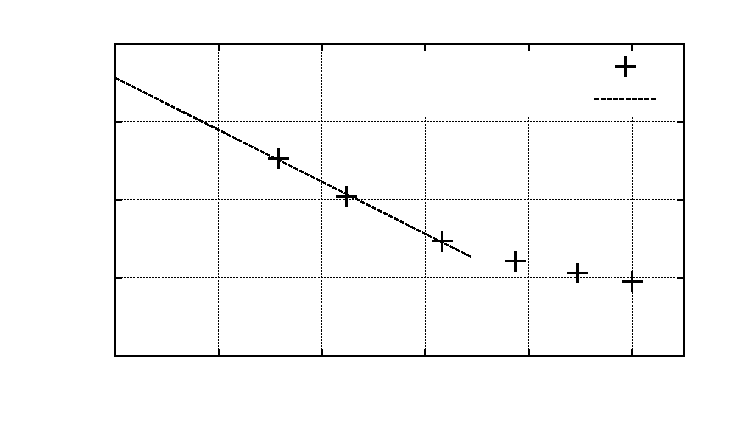
\includegraphics{lCH}}%
    \gplfronttext
  \end{picture}%
\endgroup

\caption{Závislost molární konduktivity \ce{CH_3COOH} na odmocnině z koncentrace}
\label{g:lCH}
\end{graph}

Lineární regresí závislosti molární konduktivity na odmocnině z koncentrace a následnou extrapolací pro $c_M \to 0$ jsme určili pro \ce{HCl} $\Lambda_0=\SI{37.4(2)}{\milli\siemens\metre\squared\per\mole}$ a pro \ce{CH_3COOH} $\Lambda_0=\SI{15.5(10)}{\milli\siemens\metre\squared\per\mole}$, viz diskuze.

Poznámka ke grafům: pokud je v legendě uveden vzorec některé proložené funkce, za $x$ dosazujeme číselnou hodnotu veličiny na ose x v uvedených jednotkách a získáme číselnou hodnotu veličiny na ose y v jejích jednotkách.